\section{Incident Response Fallbeispiele}

\subsection{Vorgehen wissenschaftliche Methode}
\begin{enumerate}
    \item Beobachtung/ Fragestellung
    \begin{itemize}
        \item Vorfall liegt vor
    \end{itemize}
    \item Daten sammeln
    \begin{itemize}
        \item Fortlaufendes Sammeln von Informationen zum Vorfall
    \end{itemize}
    \item Hypothese aufstellen
    \item Sofortmassnahmen aus Hypothesen ableiten und umsetzen
    \item Hypothese prüfen/ testen
    \begin{itemize}
        \item Durch Incident Response, digitale Forensik, Threat Hunting, Vulnerability Management etc. Hypothese belegen oder wiederlegen
    \end{itemize}
    \item Belegt oder wiederlegt die Prüfung/ der Test die Hypothese?
    \begin{itemize}
        \item Zusätzliche Massnahmen ableiten und umsetzten
    \end{itemize}
    \item Zurück zu Schritt 2
\end{enumerate}\grqq{}

\subsection{Hyptohesen, die wir stets annehmen}
\begin{itemize}
    \item Angreifer haben trotz aller Massnahmen immer noch Software in der Organisation für den Fernzugriff / die Fernkontrolle
    \item Angreifer setzen nicht nur selbst eingebrachte Software ein, sondern auch die bereits in der Organisation vorhandene
    \begin{itemize}
        \item Nutzerkonten kompromittiert oder neue angelegt
        \item Fernwartungswerkzeuge werden mitverwendet (Teamviewer, Anydesk etc.)
    \end{itemize}
    \item Angreifer haben Daten eingesehen / entwendet
    \item Angreifer \glqq hören und \glqq sehen\grqq{} uns zu
    \begin{itemize}
        \item Es muss immer damit gerechnet werden, dass die Angreifer die Kommunikation mitlesen können $\rightarrow$ z.B. Angreifer klinken sich ins MS-Teams des Incident Response Team ein und bekommen so alle Entdeckungen und weitere Massnahmen mit
    \end{itemize}
\end{itemize}

\subsection{Allgemeingültiges}

\subsubsection{(Technische) Ziele während der Bewältigung}
\begin{itemize}
    \item Angreifern den Zugriff in die Organisation sperren
    \begin{itemize}
        \item Organisation vom Internet trennen
        \item Strikte Netzwerksegmentierung implementieren und die Kommunikation zwischen diesen unterbinden
        \item Bekannte Command \& Control (C2) Adressen blockieren
    \end{itemize}
    \item Angreifern die Möglichkeit nehmen auf Massnahmen zu reagieren
    \item Präsenz des Angreifers aus der Organisation entfernen
    \begin{itemize}
        \item Infizierte Systeme vom Netzwerk trennen
        \item Zugriff auf kompromittierte Nutzerkonten sperren
    \end{itemize}
    \item Die Fähigkeit des Angreifers schwächen zurückzukehren
    \begin{itemize}
        \item Zugriff auf Administratorkonten einschränken
    \end{itemize}
    \item Es gibt keine Patentlösung und perfekte Reihenfolge
    \item Das Vorgehen und die Entscheidungen sind komplett vom vorhandenen Wissen abhängig
    \item Massnahmen müssen geplant, umgesetzt \underline{und überprüft/validiert} werden
    \item Falls Netzwerk offline genommen wird, muss dies überprüft werden
    \begin{itemize}
        \item an einem Client ein ping durchführen um zu überprüfen, dass wirklich keine Verbindung mehr vorhanden ist
        \item Angreifer können so oft nciht mehr machen und mithören/ mitsehen und die Incident Responder haben für die Analyse mehr Zeit
        \item kann je nach Unternehmen aber nicht komplett offline genommen werden
    \end{itemize}
\end{itemize}

\subsection{Wo fangen wir an}
\subsubsection{Ausgangspunkte}

\paragraph{E-Mail}
\begin{itemize}
    \item Empfang einer unerwünschten E-Mail, z. B. Spam, Phishing, Malspam etc.
    \item E-Mail-Header
    \begin{itemize}
        \item E-Mail-Adresse des Absenders, Quell-Server
        \item SPF, DKIM und weitere Security-Header mit wertvollen Hinweisen
    \end{itemize}
    \item Inhalt der E-Mail: Hyperlinks, Quelltext, Dateianhänge
\end{itemize}

\paragraph{Antimalware-Meldung}

\begin{itemize}
    \item Name der Schadsoftware bzw. der Detektionssignatur oder des -grundes
    \item Ort des Fundes (Dateipfad der Schadsoftware, Prozess, Netzwerkkommunikation)
    \item Hashes (Datei-Hash, Hashes bestimmter Teile der Datei (z. B. des PE Import Headers), Hashes für FuzzyMatching, )
    \item Zeitpunkt der Entdeckung oder Ausführung
    \item Aktivitäten vor/nach der Ausführung bzw. Entdeckung (EDR-Produkte)
\end{itemize}

\paragraph{Netzwerk IDS/ IPS}
\begin{itemize}
    \item Zieladresse
    \item Quelladresse / Quellsystem
    \item Kategorie der Zieladresse bzw. Grund fürs Detektieren/Blockieren
    \item Zeitpunkt des Verbindungsversuchs
\end{itemize}

\paragraph{Ransomware/ Wiper}
\begin{itemize}
    \item Neue Dateiendung der Dateien
    \item Ransom Note / Statement
\end{itemize}

\paragraph{Weitere Ausgangspunkte}
\begin{itemize}
    \item Öffentliche Angriffsfläche auf offensichtliche Schwachstellen prüfen
    \item Social Engineering
    \item Partnerorganisationen
    \begin{itemize}
        \item Sind andere Organisationen mit Vertrauensbeziehung zu unserer von einem Angriff betroffen?
        \item Site-to-Site VPN, Active Directory Trust, Fernzugriff (Teamviewer, Anydesk, persönlicher VPN etc.)
    \end{itemize}
    \item Kompromittierte Nutzerkonten
    \begin{itemize}
        \item Auffällige Anmeldungen (Ort, Uhrzeit, Software) suchen
        \item Hinweise auf Angriffe gegen Nutzerkonten (Brute-Force-Angriffe, Password Stuffing etc.)
        \item Datenlecks prüfen: Havhaveibeenpwned.com, Threat Intelligence Plattformen
    \end{itemize}
    \item Schadsoftware
    \begin{itemize}
        \item Gibt es Meldungen von AV-SW oder von IDS?
        \item Systeme mit Full-Scan prüfen
    \end{itemize}
\end{itemize}

\subsection{Indizien finden (Windows Umgebung)}

\subsubsection{Malware Paradox}
All rootkits obey two basic principles:
\begin{enumerate}
    \item They want to remain hidden
    \item They need to run
\end{enumerate}

\subsubsection{Suchmethoden}
\begin{center}
    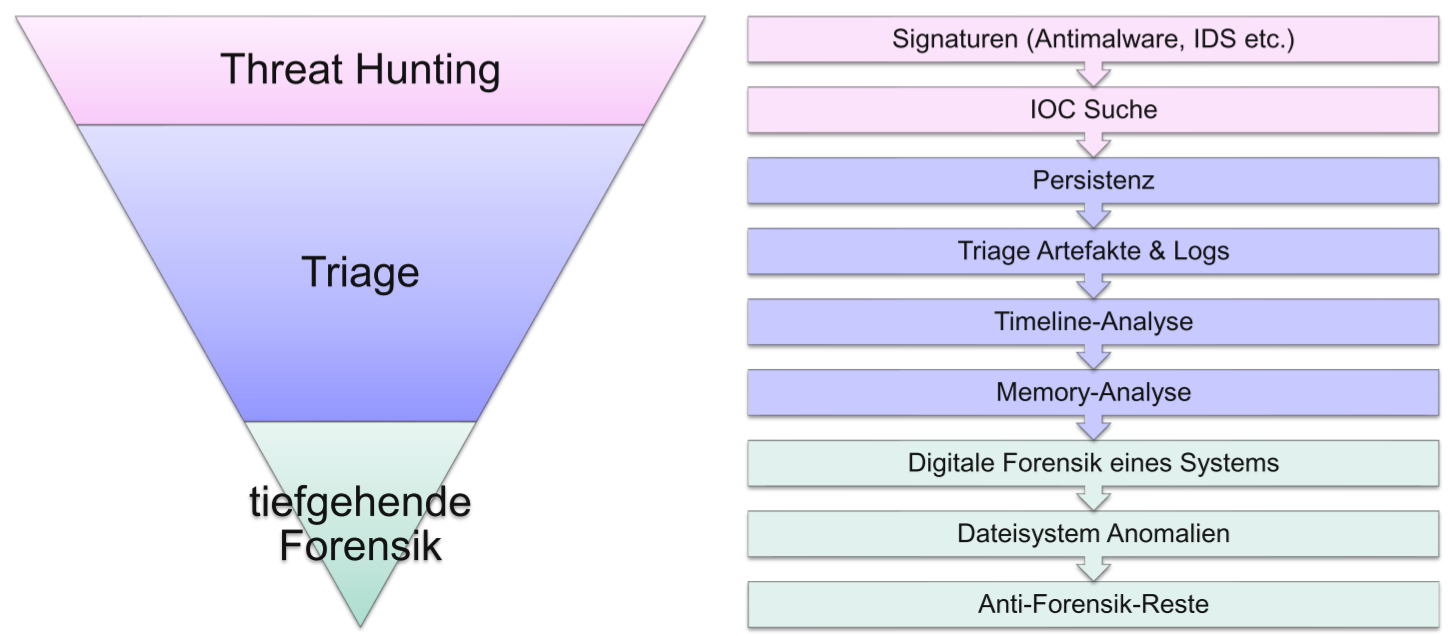
\includegraphics[width=1.0\linewidth]{07-incresp_fallbeispiele/01-suchmethoden}
\end{center}

\begin{itemize}
    \item Threat Hunting
    \begin{itemize}
        \item Suche über die gesamte Organisation
        \item Automatisierbar und skaliert gut
    \end{itemize}
    \item Triage
    \begin{itemize}
        \item Für gefundene Systeme aus der organisationsweiten Suche
        \item Prüfung auf typische Hinweise
        \item Benötigt häufig hohen manuellen Aufwand
    \end{itemize}
    \item tiefgehende Forensik (Red Poster)
    \begin{itemize}
        \item Für Systeme, die klare Hinweise auf Kompromittierung/Infektion aufweisen
        \item Sehr zeitintensiv, Vorsicht!
    \end{itemize}
\end{itemize}

\subsubsection{Angreifer versuchen nicht aufzufallen}
\begin{itemize}
    \item Schadsoftware nutzt gerne unauffällige Dateipfade oder Elemente davon
    \begin{itemize}
        \item \lstinline|\Users\%Username%\AppData\Local\Microsoft\ Windows\Temporary Internet Files|
        \item \lstinline|Temp\|
    \end{itemize}
    \item Immer Dateipfade der Prozesse überprüfen $\rightarrow$ Temp Ordner deuten tendenziell auf einen Schadprozess hin
    \item Auf ähnliche Schreibweise aufpassen
    \begin{itemize}
        \item \lstinline|winlogon| $\rightarrow$ \lstinline|wimlogom, win1ogo, winIogon, winiogon, winl0gon|
        \item \lstinline|lsass| $\rightarrow$ \lstinline|isass, laass, lamss, lass, isass, Isass|
    \end{itemize}
\end{itemize}

\subsubsection{Interesse von Lateral Movement bei IncResp}
\begin{itemize}
    \item Was wurde infiziert/ ist betroffen
    \item Auf was hat er sich fokussiert (oft Tendenz Richtung DC)?
    \item Was hat er schon erreicht (z.B. Rechte)
    \item Wie hat er sich verbreitet? $\rightarrow$ IOCs/ Massnahmen
\end{itemize}

\subsection{Triage-Akquisition}

\subsubsection{Standardprozess pro System}
\begin{enumerate}
    \item Arbeitsspeicher sichern
    \item Auf Festplattenverschlüsselung prüfen (\textit{edd.exe})
    \item Triage Image erstellen (\textit{KAPE})
    \item Analyse des Triage Image
    \begin{itemize}
        \item Vom Artefakt abhängige Analyse durchführen
    \end{itemize}
    \item Festplatten-Image erstellen
    \begin{itemize}
        \item Im Normalfall Full-Image erstellen
        \item Alternative, falls das System läuft: Logisches Image, zum Beispiel mit FTK Imager
    \end{itemize}
\end{enumerate}

\subsubsection{1. Arbeitsspeicher sichern}
\begin{itemize}
    \item Während das System noch läuft:
    \item Wenn System nicht mehr läuft:
    \begin{itemize}
        \item Hibernation-Datei: \lstinline|%SystemDrive%\hiberfil.sys|
        \item Page-Dateien: \lstinline|%SystemDrive%\pagefile.sys|
        \item Memory Dump (Crash Dumps): \lstinline|%WINDIR%\MEMORY.DMP| und \lstinline|%WINDIR%\Minidump\*.dmp|
    \end{itemize}
\end{itemize}

\subsubsection{2. Sind Festplatten verschlüsselt?}
\begin{itemize}
    \item Typisches Werkzeug: \lstinline|edd.exe|
    \begin{itemize}
        \item Organisationen sollten wissen, ob sie ihre Festplatten verschlüsseln
        \item Vorsicht, hat der Nutzer oder die Nutzerin vielleicht zusätzliche Laufwerke erstellt oder im Einsatz?
    \end{itemize}
    \item Falls verschlüsselt
    \begin{itemize}
        \item Ist der Schlüssel bekannt? $\rightarrow$ Wenn ja, notieren
        \item Falls der Schlüssel nicht bekannt ist und System noch läuft $\rightarrow$ Logisches Disk Image erstellen
    \end{itemize}
\end{itemize}

\subsubsection{3. Triage Image}
\begin{itemize}
    \item Vor dem Sammeln entscheiden, was gesammelt werden sollte
    \begin{itemize}
        \item Ausführung von KAPE \underline{hinterlässt selbst Spuren}
        \item KAPE Modules starten zusätzliche Applikationen $\rightarrow$ dies kann zum Verwischen von wertvollen Spuren führen!
    \end{itemize}
\end{itemize}

\subsection{NTFS}

\subsubsection{Wichtige NTFS-Merkmale}
\begin{itemize}
    \item Journaling (NTFS nennt es \textit{Transaction Logging}, \lstinline|$LogFile|)
    \begin{itemize}
        \item Protokolliert Änderungen an den Metadaten
        \item Tracks detailed, low-level transactional changes for NTFS
        \item Provides file system integrity and resilience (records actual data that changed)
    \end{itemize}
    \item USN Journal / Change Journal (\lstinline|$Extend\$UsnJrnl|)
    \begin{itemize}
        \item Protokolliert Änderungen an Ordnern und Dateien
        \item Nützlich für Antivirus- und Backupsoftware
        \item Tracks high-level changes
    \end{itemize}
    \item Access Control Lists
    \item Volume Shadow Copy
    \item Alternate Data Streams (ADS)
    \begin{itemize}
        \item Es können mehrere Data Streams mit einem Dateinamen in Verbindung gebracht werden
        \item Schadsoftware kann sich in diesen verstecken
    \end{itemize}
    \item Verschlüsselung (Encrypting File System, EFS)
    \begin{itemize}
        \item \underline{Nicht das gleiche wie BitLocker!}
        \item EFS \underline{verschlüsselt einzelne Dateien}, BitLocker gesamtes Laufwerk
        \item BitLocker ist unabhängig vom Nutzerkonto, EFS verschlüsselt \underline{basierend auf dem Nutzerkonto}
    \end{itemize}
\end{itemize}

\subsubsection{Master File Table (MFT), \$MFT}
\begin{itemize}
    \item Strukturiertes Array / \glqq Datenbank\grqq{} aller NTFS-Objekte
    \item Erste Einträge sind vordefiniert und für NTFS-Metadateien reserviert (Alle \lstinline|$<Files>|)
    \item Jede Datei hat mindestens einen Eintrag in der MFT mit diversen Attributen, die gespeichert werden. Unter anderem
    \begin{itemize}
        \item Grösse, Zeitstempel (\lstinline|$STANDARD_INFORMATION|), Berechtigungen
        \item Jede Datei/ Objekt haben Informationen wie Grösse, Timestamp und Berechtigungen Standardmässig vorhanden
    \end{itemize}
\end{itemize}

\subsubsection{NTFS-Metadateien}
Übersicht, welche Dateien uns helfen einen Angreifer zu finden!
\begin{center}
    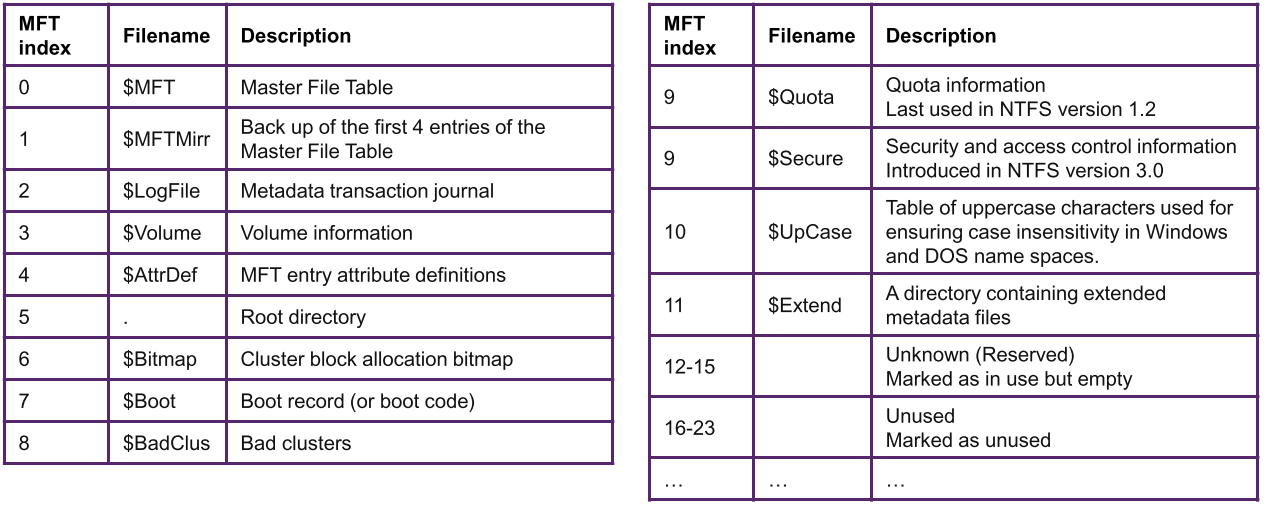
\includegraphics[width=1.0\linewidth]{07-incresp_fallbeispiele/02-ntfs_metafiles}
\end{center}

\subsubsection{Volume Shadow Copy (VSC), Volume Shadow Volumes, Volume Snapshot Service / Volume Shadow Copy Service (VSS)}
\begin{itemize}
    \item NTFS-Funktion für Backups auf Block-/Cluster-Ebene
    \item Wird manuell oder automatisch erstellt
    \item Für DFIR-Untersuchungen sehr interessant
    \begin{itemize}
        \item Kann vermeintlich gelöschtes wiederherstellbar machen
        \item Kann einen weiteren Blick in die Vergangenheit erlauben (Logs, Prefetch, LNKs etc.)
    \end{itemize}
    \item Oft gehen die VSS vergessen
\end{itemize}

\subsection{Windows Registry}

\subsubsection{Registry Hives}
Ein Hive in der Windows-Registry ist die Bezeichnung für einen Hauptbereich der Registry, der Informationen als Key-Value-Pair enthält.

Alle Schlüssel, die als Hives gelten, beginnen mit \textit{HKEY} und befinden sich an der Registry-Root.

\subsubsection{Security Accounts Manager (SAM)}
\begin{itemize}
    \item SAM Hive gibt uns Informationen zu \underline{lokalen} Nutzerkonten
    \begin{itemize}
        \item wenn Nutzerkonten Teil einer Windows Domäne sind, dann sind die Informationen zu den Nutzerkonten auf den Domain-Controller-Systemen
    \end{itemize}
    \item DFIR-Relevanz:
    \begin{itemize}
        \item Nutzername zum Relative Identifier (RID, letzter Teil vom SID) identifizieren
        \item Nutzerverhalten aus erfolgreichen und fehlgeschlagenen Anmeldeversuchen ableiten
        \item Vorsicht: Bei Microsoft Nutzerkonen (SaaS/Cloud) werden die Counter \underline{nicht} genutzt
        \item Diverse Zeitstempel für Korrelation und Identifikation potenziell verdächtiger Nutzerkonten
    \end{itemize}
\end{itemize}

\subsubsection{Zeitzone}
\begin{itemize}
    \item Bei jedem Zeitstempel müssen wir die Zeitzone kennen
    \item Wenn möglich immer mit \textbf{UTC} arbeiten
    \item Gewisse Logs und Dateisystem (z. B. FAT) nutzen die lokal eingestellte Zeitzone
\end{itemize}

\subsection{E-Mail Analyse}

\subsubsection{E-Mail Header}
\begin{itemize}
    \item \textbf{Wichtig}: Der Grossteil der E-Mail-Header lassen sich fälschen!
    \begin{itemize}
        \item Einzig dem letzten E-Mail-Server, unserem eigenen, können wir (hoffentlich) vertrauen und damit den von ihm eingefügten Header
    \end{itemize}
    \item Jeder Mailserver der die E-Mail passiert fügt im Normalfall Header hinzu (ganz oben)
    \item MTA: Mail Transfer Agent ist zuständig für das entgegennehmen und senden von E-Mails
    \begin{itemize}
        \item MUA: Mail User Agent ist die Software zur Bearbeitung von E-Mails (E-Mail-Client)
        \item MDA: Mail Delivery Agent ist zuständig für die Bereitstellung der E-Mails an den MUA verantwortlich
        \item MTA $\leftrightarrow $ MTA, MTA $\rightarrow$ MDA und MUA $\rightarrow$  MTA meist über SMTP
        \item MDA $\rightarrow$ MUA meist IMAP (früher POP)
    \end{itemize}
\end{itemize}

\begin{center}
    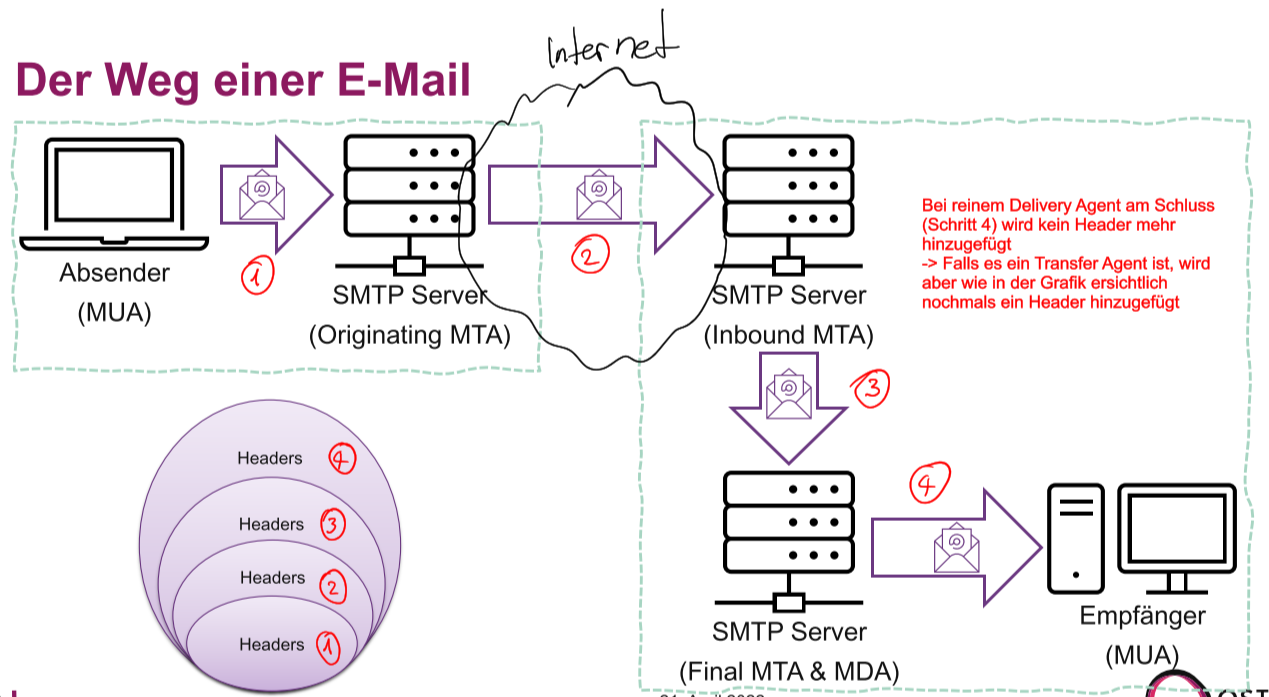
\includegraphics[width=1.0\linewidth]{07-incresp_fallbeispiele/03-email}
\end{center}

\subsubsection{Typische Header-Felder}
\begin{itemize}
    \item \textbf{Message-ID}: [Eindeutige ID]@[Originating MTA]
    \begin{itemize}
        \item Eindeutige Identifikation für die E-Mail
        \item Erlaubt beispielsweise die Suche nach Protokollereignissen im Zusammenhang mit der E-Mail
    \end{itemize}
    \item \textbf{Received}
    \begin{itemize}
        \item Erlaubt es den Weg des E-Mails zu verfolgen (von unten nach oben)
        \item Der \textcolor{red}{unterste Eintrag} ist der \textcolor{red}{Originating MTA} und der \textcolor{OSTPink}{oberste Eintrag} ist der \textcolor{OSTPink}{Final MTA}
        \item Jeder MTA fügt im Normalfall die eigene \textit{IP-Adresse}, seinen eigenen \textit{Namen}, die \textit{Quell-IPAdresse}, den Namen des \textit{Quellsystems} und den \textit{Empfangszeitpunkt inkl. Zeitzone} hinzu
    \end{itemize}
    \item \textbf{X-Originating-IP, X-IP, X-Forwarded-For}
    \begin{itemize}
        \item Kann existieren und die IP-Adresse des Absenders (MUA) enthalten
        \item Müssen dafür dem Originating MTA vertrauen
        \item Immer seltener vorhanden zum Schutz der Privatsphäre bzw. wegen Datenschutzbedenken
    \end{itemize}
\end{itemize}

\subsubsection{SPF (Sender Policy Framework)}
Mit \textit{SPF} können Absender festlegen, welche IP-Adressen E-Mails für eine bestimmte Domäne senden dürfen.
DNS TXT-Entry mit allen IP-Ranges, von welchen ein Mail mit dieser Domain verschickt werden darf.
Alles was nicht von den outgoing Mail/MX Servern stammt, ist ''Fake''und wird in Spam verschoben oder gar nicht erst zugestellt.\\

\textit{SPF} ist besonders effizient gegen \textcolor{red}{\textbf{Phishing-Angriffe}} \& erlaubt es dem Empfänger gefälschte Absender festzustellen.

\subsubsection{Ablauf}
Auf dem \textbf{DNS} kann eingegrenzt werden, wer (welche IP) alles ein Mail verschicken darf.
\begin{itemize}
    \item \textcolor{purple}{\textbf{MTA}} macht \textbf{DNS-Lookup} und fragt diesen an, welche IPs berechtig sind Mails zu versenden.
    \begin{itemize}
        \item IP-$\alpha$ (TCP) $\rightarrow$ DNS-Lookup $\rightarrow$ SPF@ost.ch
        \item Falls $\alpha$ darin enthalten $\rightarrow$ ok
    \end{itemize}
\end{itemize}

Wenn Empfänger SPF-Policy nicht enforced, ist egal was der Sender konfiguriert hat. Empfänger-MTA interessiert das nicht.\\

\subsubsection{DKIM (DomainKeys Identified Mail)}
\textcolor{cyan}{\textbf{DKIM}} stellt einen Encryption Key und eine digitale Signatur bereit, die nachweisen, dass eine E-Mail-Nachricht nicht gefälscht oder verändert wurde.
DKIM fügt dazu dem E-Mail Header eine digitale Signatur hinzu, welche vom Empfänger mit dem \textit{Public Key} (welcher auf dem DNS Server gespeichert ist) validiert werden kann.\\

Der Mail-Server hat ein Public/Private Key Cert Pair. Der Public Key wird via weltweit verfügbaren DNS veröffentlicht. 
Der Plaintext in einem Mail wird gehasht und im Header gespeichert. 
Der Header wird wieder mit dem Private Key signiert (also inkl. dem Hash des Plain Texts). 
Empfänger Mail-Server kann nun mit dem öffentlich verfügbaren Public Key feststellen, ob der Sender der ist der er angibt (Korrekte Firma mit Zugriff auf Private/Public Pair). 
Durch das Signieren ist auch klar, dass der Content ''in Transit'' nicht verändert wurde.\\

\textit{DKIM} ist besonders effizient gegen \textcolor{red}{\textbf{Man-in-the-middle-Angriffen}}.

\subsubsection{Ablauf}
\begin{itemize}
    \item Mailserver signiert Mail mit private Key
    \item Mail kommt beim  \textcolor{purple}{MTA} an und dieser prüft ob Mail signiert ist
    \begin{itemize}
        \item Wenn Signatur vorhanden $\rightarrow$ \textbf{DNS-lookup} für public key $\rightarrow$ prüft Signatur von Mail mit dem public key des \textbf{DNS Servers}\\
    \end{itemize}
\end{itemize}

\paragraph{Canonicalization}
\begin{itemize}
    \item Während dem Transport werden E-Mails verändert
    \item Canonicalization \underline{normalisiert} die E-Mail mit dem Ziel, dass Änderungen während dem Transport \underline{keinen negativen Effekt auf die Validierung der Signatur} haben
\end{itemize}

\paragraph{DFIR}
\begin{itemize}
    \item Indikator, dass bestimmte Header-Felder und/oder E-Mail-Inhalt nicht verändert wurden zwischen dem MTA des Absenders (Absender vertraut diesem) und unserem MTA (wir vertrauen diesem).
    \item \lstinline|Authentication-Results| ist das Resultat der Signaturprüfung durch den MTA auf der Empfangsseite. Enthält im \lstinline|header.b| die ersten 8 Bytes der Signatur
\end{itemize}

\subsubsection{(Versteckte) Zeitstempel in E-Mails}
\begin{itemize}
    \item Offensichtliche Zeitstempel: \lstinline|X-Received, Received, Date|
    \item Abweichung von Zeit $\rightarrow$ Indicator
    \begin{itemize}
        \item Könnte aber auch sein, dass Admin Zeit falsch eingestellt oder Server geografisch verschoben wurde (ohne Zeit anzupassen) und kein NTP Server konfiguriert ist
    \end{itemize}
    \item Weniger offensichtlich: Unix Timestamps können an diversen Orten versteckt sein
\end{itemize}

\subsection{Windows Event Logs}

\subsubsection{Security Log}
\begin{itemize}
    \item \textbf{Wichtigstes} Log bei DFIR-Analysen
    \item Nur der LSASS-Prozess darf in diesen schreiben (Nur Admins können diese sehen)
    \item Logeinträge werden durch die Audit Policy gesteuert (können spezifisch für einzelne Benutzerkonten eingestellt werden)
    \item Details zu Authentifizierung, Nutzerverhalten, Zugriff auf Ressourcen (Dateien, Ordner, Netzwerklaufwerke/-ordner), Änderungen an gewissen Einstellungen etc.
\end{itemize}

\subsubsection{Nutzerkontonutzung}
\begin{itemize}
    \item \textbf{Anmeldeversuche überwachen/ Audit account logon events}
    \begin{itemize}
        \item Bestimmt, ob jede Instanz eines Benutzers überwacht werden soll, der sich bei einem \underline{anderen} Gerät anmeldet oder sich von einem anderen Gerät abmeldet, auf dem \underline{dieses} Gerät zum Überprüfen des Kontos verwendet wird.
        \item Anmelde-/Abmeldeereignisse, die auf dem untersuchten System authentifiziert werden.
        \item Es ist aber \underline{nicht} (zwingend) das System an dem sich eine Person anmeldet.
    \end{itemize}
    \item \textbf{Anmeldeereignisse überwachen/ Audit logon events}
    \begin{itemize}
        \item Bestimmt, ob jede Instanz eines Benutzers überwacht werden soll, der sich bei einem Gerät anmeldet oder sich von einem Gerät abmeldet.
        \item Anmelde-/Abmeldeereignisse, die auf dem System selbst stattfinden
    \end{itemize}
\end{itemize}

\subsubsection{Logon Type}
\begin{center}
    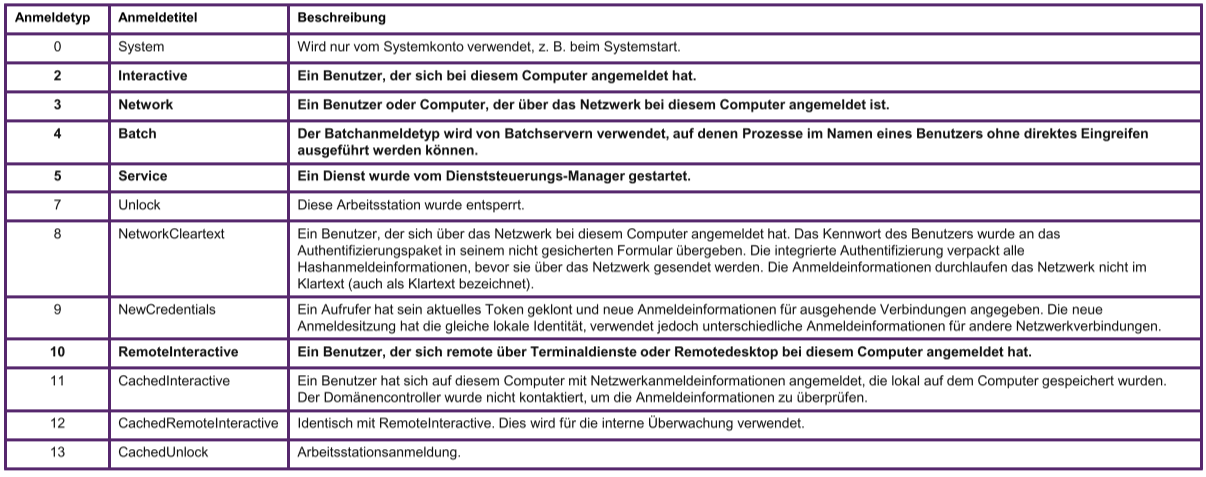
\includegraphics[width=1.0\linewidth]{07-incresp_fallbeispiele/04-eventlog_logontype}
\end{center}

\subsubsection{Anmeldesitzung nachverfolgen}
Je nach dem wie viele Tätigkeiten während der aktiven Sitzung ausgeführt wurden kann auf eine Automatisation geschlossen werden oder nicht. \\
$\rightarrow$ Duzende Tätigkeiten (Service installiert, Scheduled Task erstellt, etc.) in 3 Min $\rightarrow$ Automation

\subsection{Browser}
\begin{minipage}{0.6\linewidth}
    \paragraph{Fragen}
    \begin{itemize}
        \item Welche Webseite wurde besucht?
        \item Wie häufig wurde die Webseite besucht?
        \item Wann wurde eine Webseite besucht?
        \item Welche Webseiten hat sich der Nutzer/die Nutzerin gemerkt?
        \item Was wurde heruntergeladen?
        \item Welche Nutzerkonten wurden online verwendet?
        \item Nach was wurde gesucht?
    \end{itemize}
    \vfill
    $ $
\end{minipage}
\begin{minipage}{0.4\linewidth}
    \paragraph{Artefakte zur Beantwortung}
    \begin{itemize}
        \item Browser-Verlauf
        \item Cache
        \item Cookies
        \item Sitzungswiederherstellung
        \item Autovervollständigung
        \item Favoriten
        \item Download-Historie
        \item (Sync-)Einstellungen
    \end{itemize}
\end{minipage}

\subsubsection{In die Tiefen der Browser steigen}
\begin{itemize}
    \item Für tiefgehende Analysen fehlt häufig die Zeit (abhängig von Browser + sehr viele Informationen fürs Auswerten)
    \item Im IR setzen wir häufig auf alternative Quellen für Hinweise:
    \begin{itemize}
        \item Logs (DNS, FW, AV)
        \item Dateien im Downloads-Ordner oder Papierkorb des Systems
        \item E-Mail-Server (E-Mail häufig der Ausgangspunkt einer unerwünschten Browser-Nutzung)
    \end{itemize}
\end{itemize}